\renewcommand*{\arraystretch}{1.1}

\subsection*{Interactive / complex / 12}
\label{section:interactive-complex-read-12}

% change \emph{} to use sans-serif font
\let\oldemph\emph
\renewcommand{\emph}[1]{{\footnotesize \sf #1}}

\renewcommand{\currentQueryCard}{12}
\marginpar{
	\raggedleft
	\vspace{0.22ex}

	\queryRefCard{interactive-complex-read-01}{IC}{1}\\
	\queryRefCard{interactive-complex-read-02}{IC}{2}\\
	\queryRefCard{interactive-complex-read-03}{IC}{3}\\
	\queryRefCard{interactive-complex-read-04}{IC}{4}\\
	\queryRefCard{interactive-complex-read-05}{IC}{5}\\
	\queryRefCard{interactive-complex-read-06}{IC}{6}\\
	\queryRefCard{interactive-complex-read-07}{IC}{7}\\
	\queryRefCard{interactive-complex-read-08}{IC}{8}\\
	\queryRefCard{interactive-complex-read-09}{IC}{9}\\
	\queryRefCard{interactive-complex-read-10}{IC}{10}\\
	\queryRefCard{interactive-complex-read-11}{IC}{11}\\
	\queryRefCard{interactive-complex-read-12}{IC}{12}\\
	\queryRefCard{interactive-complex-read-13}{IC}{13}\\
	\queryRefCard{interactive-complex-read-14}{IC}{14}\\
}


\noindent\begin{tabularx}{\queryCardWidth}{|>{\queryPropertyCell}p{\queryPropertyCellWidth}|X|}
	\hline
	query & Interactive / complex / 12 \\ \hline
%
	title & Expert search \\ \hline
%
	pattern & \centering 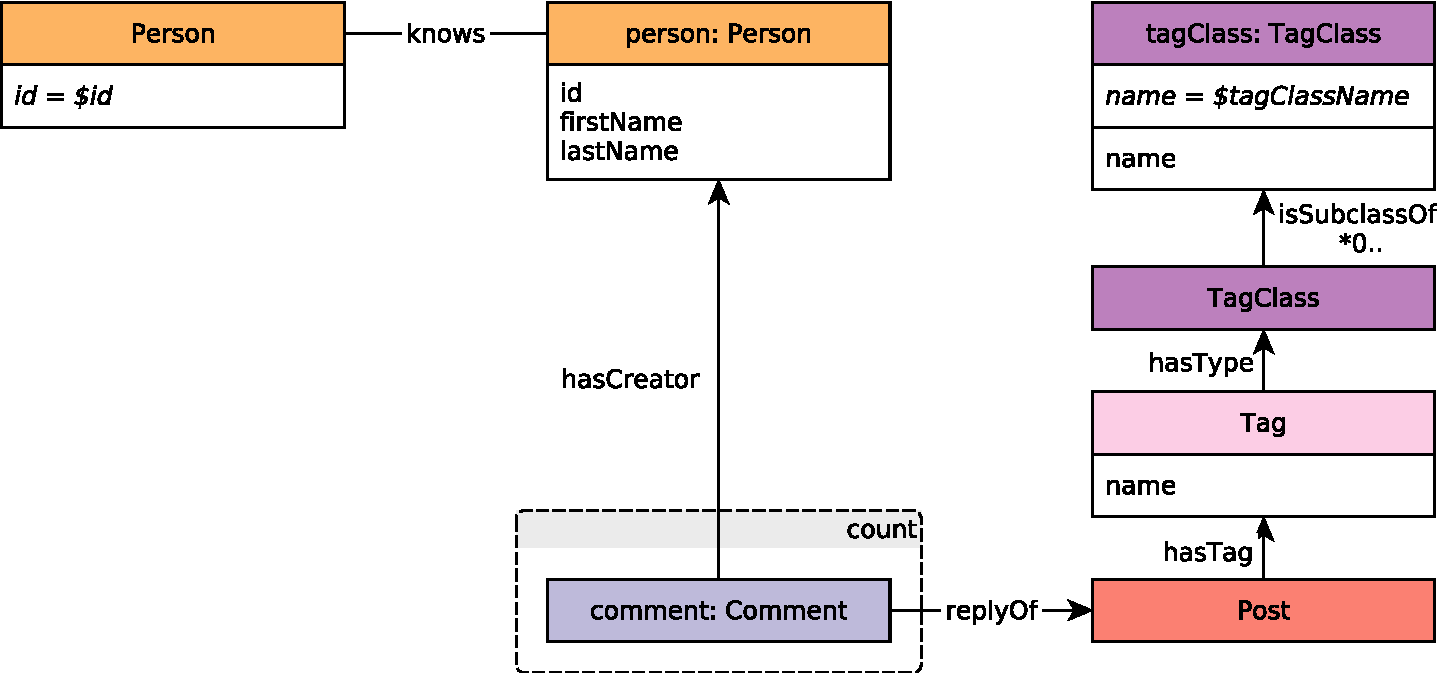
\includegraphics[scale=\patternscale,margin=0cm .2cm]{patterns/interactive-complex-read-12} \tabularnewline \hline
%
	desc. & Given a start \emph{Person}, find the \emph{Comments} that this
\emph{Person}'s friends made in reply to \emph{Posts}, considering only
those \emph{Comments} that are direct (single-hop) replies to
\emph{Posts}, not the transitive (multi-hop) ones. Only consider
\emph{Posts} with a \emph{Tag} in a given \emph{TagClass} or in a
descendent of that \emph{TagClass}. Count the number of these reply
\emph{Comments}, and collect the \emph{Tags} that were attached to the
\emph{Posts} they replied to, but only collect \emph{Tags} with the
given \emph{TagClass} or with a descendant of that \emph{TagClass}.
Return \emph{Persons} with at least one reply, the reply count, and the
collection of \emph{Tags}.
 \\ \hline
%
	
		params &
		\innerCardVSpace{\begin{tabularx}{\attributeCardWidth}{|>{\paramNumberCell}c|>{\varNameCell}M|>{\typeCell}m{\typeWidth}|Y|} \hline
		$\mathsf{1}$ & Person.id
 & ID
 & \texttt{personId}
 \\ \hline
		$\mathsf{2}$ & TagClass.name
 & String
 & \texttt{tagClassName}
 \\ \hline
		\end{tabularx}}\innerCardVSpace \\ \hline
	
%
	
		result &
		\innerCardVSpace{\begin{tabularx}{\attributeCardWidth}{|>{\resultNumberCell}c|>{\varNameCell}M|>{\typeCell}m{\typeWidth}|>{\resultOriginCell}c|Y|} \hline
		$\mathsf{1}$ & Person.id & ID & R &
				\texttt{personId}
 \\ \hline
		$\mathsf{2}$ & Person.firstName & String & R &
				\texttt{personFirstName}
 \\ \hline
		$\mathsf{3}$ & Person.lastName & String & R &
				\texttt{personLastName}
 \\ \hline
		$\mathsf{4}$ & \{Tag.name\} & \{String\} & R &
				\texttt{tagNames}
 \\ \hline
		$\mathsf{5}$ & replyCount & 32-bit Integer & A &
				\texttt{replyCount} -- Number of reply Comments
 \\ \hline
		\end{tabularx}}\innerCardVSpace \\ \hline
	
%
	
		sort		&
		\innerCardVSpace{\begin{tabularx}{\attributeCardWidth}{|>{\sortNumberCell}c|>{\varNameCell}M|>{\directionCell}c|Y|} \hline
		$\mathsf{1}$ & count
 & $\desc
$ &  \\ \hline
		$\mathsf{2}$ & Person.id
 & $\asc
$ &  \\ \hline
		\end{tabularx}}\innerCardVSpace \\ \hline
	%
	limit & 20 \\ \hline
	%
	CPs &
	\multicolumn{1}{>{\raggedright}l|}{
		\chokePoint{3.3}, 
		\chokePoint{7.2}, 
		\chokePoint{7.3}, 
		\chokePoint{8.2}
		} \\ \hline
	%
	relevance &
		\footnotesize This query looks for paths of length three, starting at a *Person*, moving to its friends, the to their *Comments* and ending at the *Post* the *Comments* are replying. The chain from original post to the reply is transitive. The traversal may be initiated at either end, the system may note that this is a tree, hence leaf to root is always best. Additionally, a hash table can be built from either end, e.g. from the friends of self, from the tags in the category, from the or other.
 \\ \hline%
\end{tabularx}
\queryCardVSpace

% change \emph back to the old one
\let\emph\oldemph